\section{Architecture of the Tokenizer}

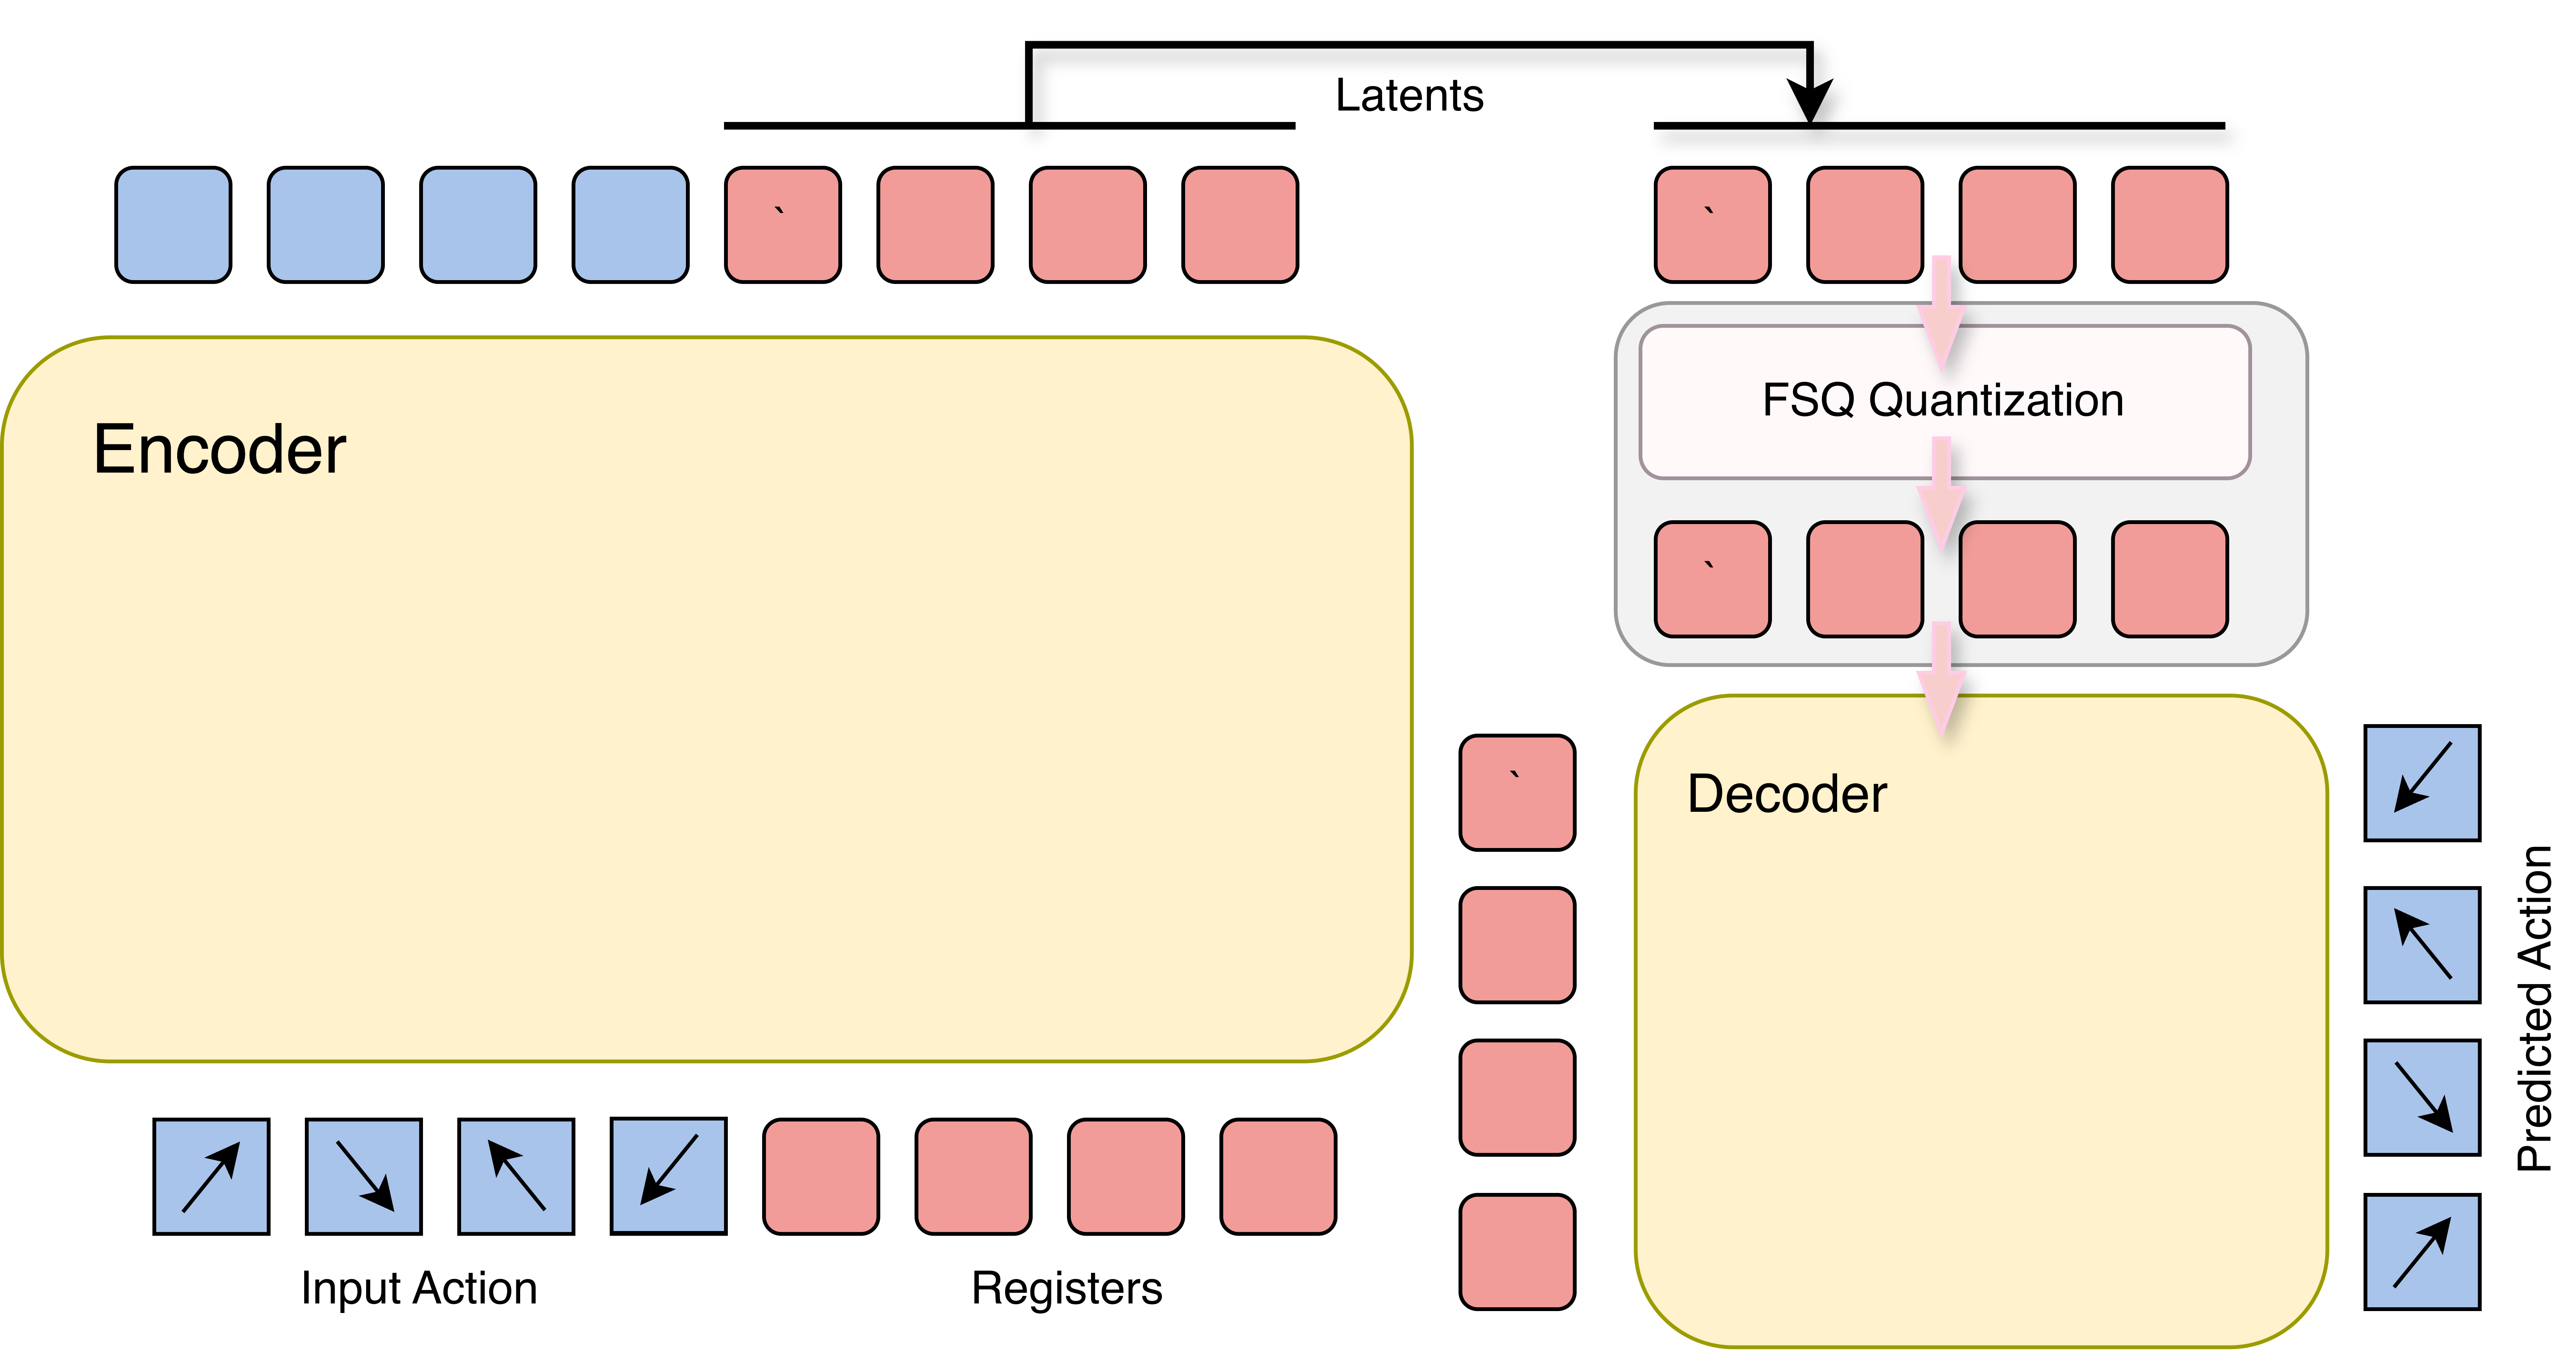
\includegraphics[width=\linewidth]{Ttokenization_v2.png}

It is generally accepted that the reconstruction quality
of a tokenizer is not necessarily indicative of the success
of the downstream generative model. We find that it is
equally important to distribute information appropriately
across the token space. This motivates our tokenizer
architecture, where compression and information allocation
are the primary objectives, rather than the sharpness of
the reconstruction. In particular, we argue that less smooth
motions with higher jerk provide a worse inductive bias
for autoregressive policies.

A 1D tokenizer can be viewed as a variant of tokenization
in which the latent tokens need not correspond to individual
timesteps or follow a fixed temporal ordering. We therefore
consider a simple architecture that allows us to represent
an action sequence using an unordered set of latent tokens.
Our architecture is inspired by the recent work
TiTok~\cite{titok}.

Specifically, we introduce a set of learnable embeddings,
which are concatenated with the action embeddings and
processed to obtain latent representations. We then apply
finite scalar quantization (FSQ) to these latents to obtain
discrete tokens.

The discrete latents are subsequently passed through a
cross-attention module with another set of learnable
embeddings. The resulting representations are then processed
by a Transformer decoder to reconstruct the original
action sequence.
